\documentclass[twocolumn]{el-author}

%\usepackage[...]{...}      This has been commented out as we are not using any additional packages here.  On the whole, they should be unnecessary.
\newcommand{\hH}{\hat{H}}
\newcommand{\D}{^\dagger}
\newcommand{\ua}{\uparrow}
\newcommand{\nc}{\newcommand}
\nc{\da}{\downarrow} \nc{\hc}{\hat{c}} \nc{\hS}{\hat{S}}
\nc{\bra}{\langle} \nc{\ket}{\rangle} \nc{\eq}{equation (\ref}
\nc{\h}{\hat} \nc{\hT}{\h{T}}\nc{\be}{\begin{eqnarray}}
\nc{\ee}{\end{eqnarray}}\nc{\rd}{\textrm{d}}\nc{\e}{eqnarray}\nc{\hR}{\hat{R}}\nc{\Tr}{\mathrm{Tr}}
\nc{\tS}{\tilde{S}}\nc{\tr}{\mathrm{tr}}\nc{\8}{\infty}\nc{\lgs}{\bra\ua,\phi|}\nc{\rgs}{|\ua,\phi\ket}
\nc{\hU}{\hat{U}}\nc{\lfs}{\bra\phi|}\nc{\rfs}{|\phi\ket}\nc{\hZ}{\hat{Z}}\nc{\hd}{\hat{d}}\nc{\mD}{\mathcal{D}}
\nc{\bd}{\bar{d}}\nc{\bc}{\bar{c}}\nc{\mc}{\mathcal}\nc{\ea}{eqnarray}\nc{\mG}{\mathcal{G}}\nc{\bce}{\begin{center}}
\nc{\ece}{\end{center}}
\date{4th February 2016}

\begin{document}

\title{This Hypergraph Partitioning is to Awesome for You to Handle}

\author{Foo and Bar}

\abstract{DAT ABSTRACT.}

\maketitle

\section{State of the Art}

\subsection{VLSI Design Flow}
\begin{figure}[h]
\centering{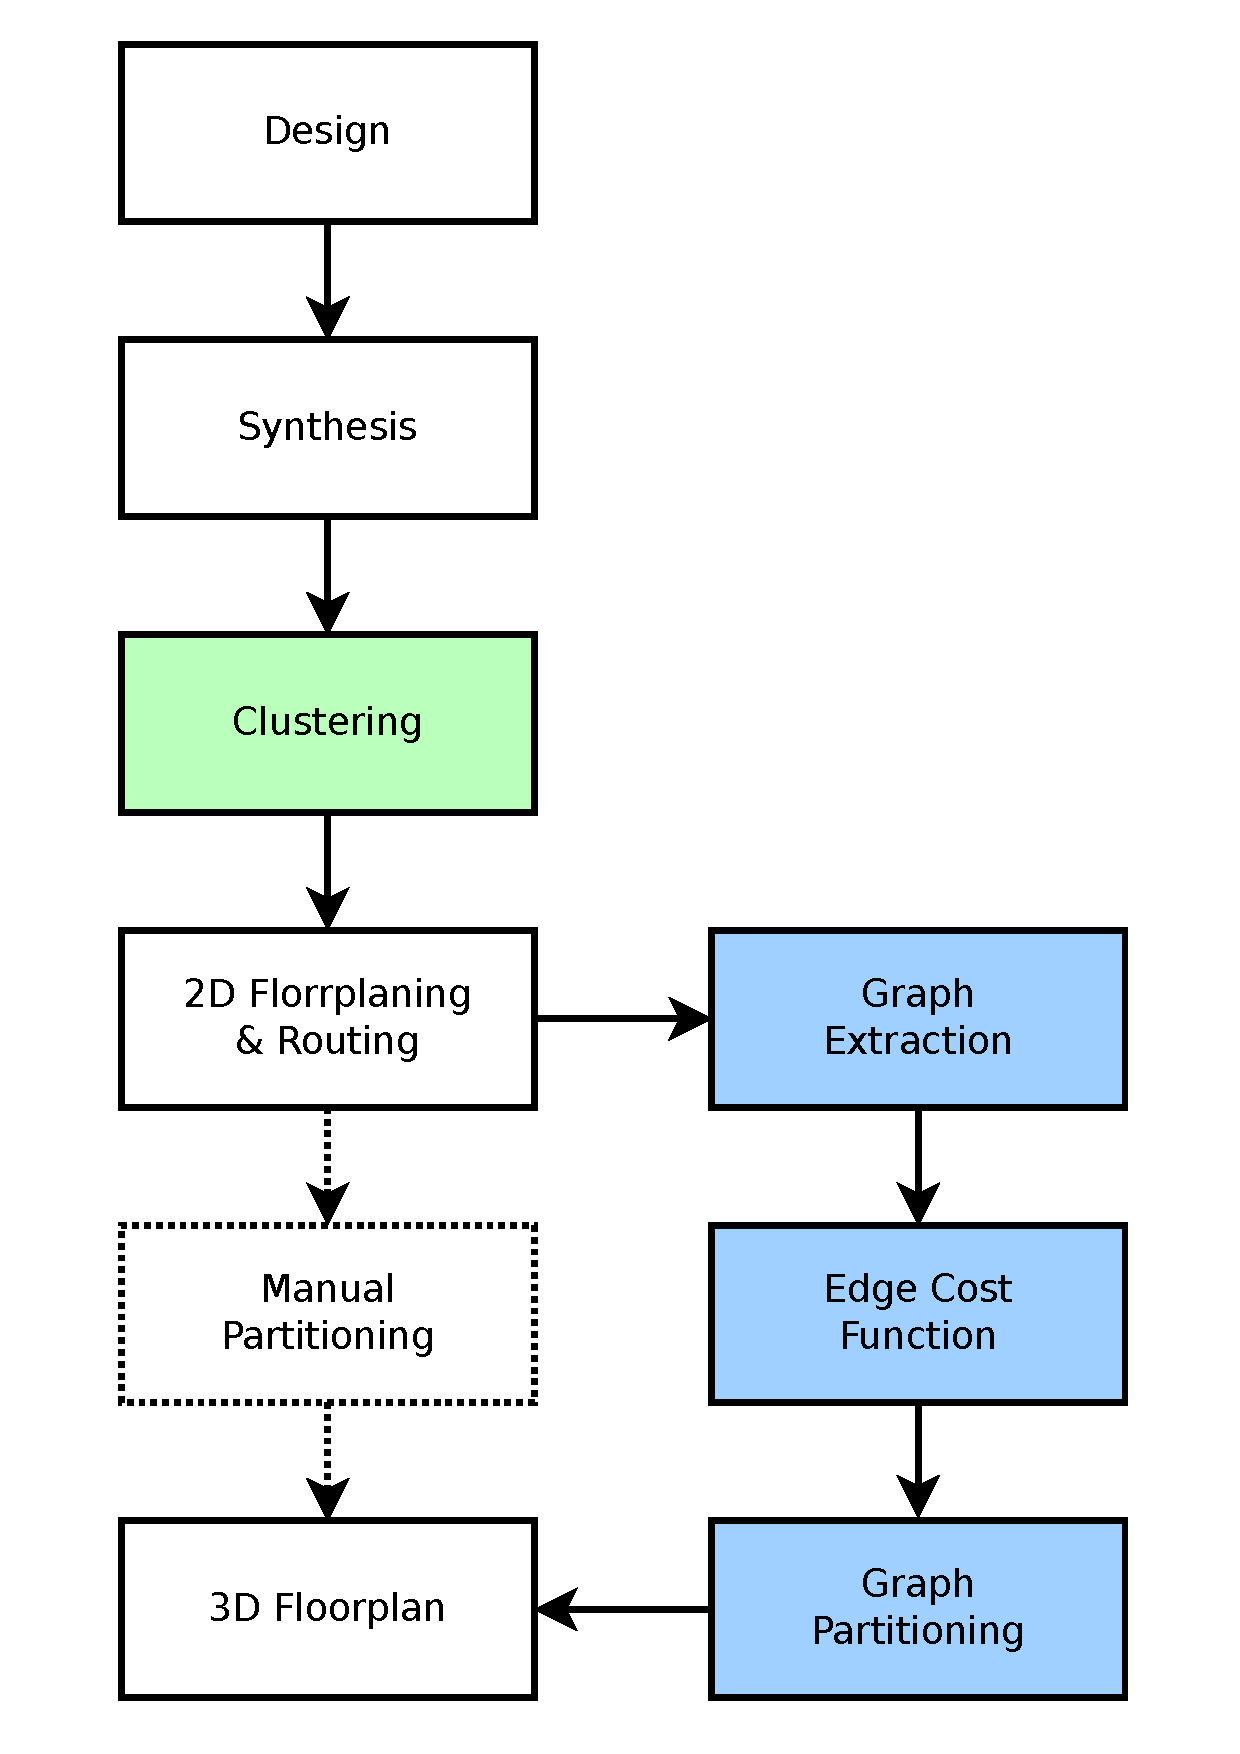
\includegraphics[width=60mm]{design-flow}}
\caption{Modified design flow including the 3D partitioning (in blue).}
\end{figure}

\subsection{Graph Partitioning}
Graph partitioning is an NP-hard problem\footnote{Cite the book from INFOF402?}.
As such, heuristics are used to extract an approximated solution in a finite amount of time.

\subsection{Hypergraph}

\subsection{Multilevel partitioning}
\subsubsection{Coarsening Phase}

\subsubsection{Initial Partitioning}
\begin{itemize}
  \item Kernighan-Lin
  \item Fiduccia-Mattheyses
\end{itemize}


\subsubsection{Uncoarsening phase}

% \begin{thebibliography}{}
%
% \bibitem{1}
% Anderson, P.: `A poor man's derivation of scaling laws for the Kondo problem', \textit{J. Phys. C.}, 1960, \textbf{3}, p. 2436
%
% \bibitem{2}
% Coleman, P.: `1/N expansion for the Kondo lattice', \textit{Phys. Rev. B}, 1983, \textbf{28}, pp. 5255-5262
%
% \bibitem{3}
% Ludwig, I. and Ludwig A. W. W.: `Kondo effect induced by a magnetic field', \textit{Phys. Rev. B}, 2001, \textbf{64}, p. 045328
%
% \end{thebibliography}

\end{document}

%\begin{table}[b]
%\processtable{Coefficients and remainders for distribution KK ($k = 0.05$,
%$v = 3$, $c_{1} = 1.5$, $c_{2} = 4.5$)}
%{\begin{tabular}{|l|l|l|}\hline
%$n$ & $a_{n}^{2}$ & $r_{k}(1)$\\\hline
%0 & 3.602576748428 & 1.493719547999\\\hline
%1 & 1.384791111989 & 0.108928436101\\\hline
%2 & 0.108600438794 & 0.000327997399\\\hline
%3 & 0.000275794597 & 0.000052202814\\\hline
%4 & 0.000027616892 & 0.000024585922\\\hline
%5 & 0.000018178621 & 0.000006407300\\\hline
%\end{tabular}}{}
%\end{table}
%
%So, the basic preamble and main body will be:
%\verb"\documentclass[twocolumn]{el-author}"\\
%\verb"\usepackage[...]{packages}"\\
%\verb"\date{12 December 2012}"\\
%\verb"\title{...}"\\
%\verb"\author{...}"\\
%\verb"\abstract{...}"\\
%\verb"\maketitle{...}"\\
%\verb"\begin{document}"\\
%\verb"..."\\
%\verb"\section{...}"\\
%\verb"..."\\
%\verb"\section{..}"\\
%\verb"..."\\
%\verb"\end{document}"
